% Auriga theme
% https://github.com/anishathalye/auriga

\documentclass[14pt,aspectratio=169]{beamer}
\usepackage{pgfpages}
\usepackage{fancyvrb}
\usepackage{booktabs,dcolumn}
\usepackage{tikz}
\usetikzlibrary{arrows.meta, positioning, quotes}
\usepackage{pgfplots}

% \ifnotes
% \setbeamertemplate{note page}[plain]
% \setbeameroption{show notes on second screen=right}
% \fi

\usetheme{auriga}
\usecolortheme{auriga}

% define some colors for a consistent theme across slides
\definecolor{red}{RGB}{181, 23, 0}
\definecolor{blue}{RGB}{0, 118, 186}
\definecolor{gray}{RGB}{146, 146, 146}

\title{Historia Económica Argentina}

\author{\underline{Sebastián Freille} \inst{1}}

\institute[shortinst]{\inst{1} IEF-UNC \\ UCC}
\date{}

\AtBeginSection[]{
    \begin{frame}
    \vfill
    \centering
    \begin{beamercolorbox}[sep=8pt,center,shadow=true,rounded=true]{title}
        \usebeamerfont{title}\insertsectionhead\par%
    \end{beamercolorbox}
    \vfill
    \end{frame}
}



\AtBeginSubsection[]{
    \begin{frame}
    \vfill
    \centering
    \begin{beamercolorbox}[sep=6pt,center,shadow=true,rounded=true]{title}
        \usebeamerfont{title}\insertsubsectionhead\par%
    \end{beamercolorbox}
    \vfill
    \end{frame}
}


\AtBeginSubsubsection[]{
    \begin{frame}
    \vfill
    \centering
    \begin{beamercolorbox}[sep=4pt,center,shadow=true,rounded=true]{title}
        \usebeamerfont{title}\insertsubsubsectionhead\par%
    \end{beamercolorbox}
    \vfill
    \end{frame}
}


\begin{document}


{
  % rather than use the frame options [noframenumbering,plain], we make the
  % color match, so that the indicated page numbers match PDF page numbers
  \setbeamercolor{page number in head/foot}{fg=background canvas.bg}
  \begin{frame}
    \titlepage
  \end{frame}
}

  
  \section{Capítulo 1. El período de progreso}

  \subsection{Sistema monetario: Pre-Caja de Conversión}


  \begin{frame}\frametitle{La cuestión monetaria en un país con BPE}
     \begin{itemize}
\item ¿Cómo juega el dinero --en sus diferentes formas- y el crédito
  en una economía en expansión?
  \item ¿Existe una relación entre el crecimiento de la economía y el
    crecimiento del dinero?
     \item ¿Se puede mantener la convertiblidad de la moneda?
       \item ¿Por qué se abandona la convertibilidad
         monetaria en el caso que se haga?
                 \end{itemize}
        \end{frame}

  
\begin{frame}\frametitle{Sistemas monetarios: Historia}
     \begin{itemize}
     \item Anarquía monetaria $\longrightarrow$ antes de 1880
       \item Unificación monetaria $\longrightarrow$
         entre 1881 y 1891
       \item Caja de Conversión $\longrightarrow$ 1891 a 1935
         (inactiva 1914-1927)
         \item Creación de Banco Central $\longrightarrow$ 1935-actualidad
         \end{itemize}
        \end{frame}

        
% \begin{frame}\frametitle{Sistemas monetarios: Historia}
%      \begin{itemize}
%      \item Año 1867-76 $\longrightarrow$ 
%        \item Año 1881 $\longrightarrow$ unificación monetaria (Ley 1130)
%        \item Años 1883-85 $\longrightarrow$ convertibilidad monetaria
%          entre peso papel y peso oro
%          (patrón oro)
%          \item Años 1885-1887 $\longrightarrow$ suspensión de
%            convertibilidad
%            \item Año 1887 $\longrightarrow$ Bancos Nacionales
%              Garantidos
%              \item Años 1900-1913 $\longrightarrow$ 
%          \end{itemize}
%         \end{frame}


 \begin{frame}\frametitle{Convertibilidad}
     \begin{block}{¿Que es la convertibilidad?}
    Convertibilidad implica que el dinero papel es convertible
    legalmente a moneda dura --divisa externa u oro (metal). En
    teoría, implica el respaldo al 100\% (o menos) de la emisión
    monetaria en la moneda dura. Si la conversión es al 100\%, la
    única fuente de emisión monetaria es por saldos comerciales
    favorables y/o entrada de capitales. Si la conversión es al menos
    del 100\%, entonces hay lugar para otras fuentes de emisión
    --préstamos al Estado, redescuentos de documentos comerciales.  
       \end{block}
        \end{frame}
        

        \begin{frame}\frametitle{Convertibilidad a traves de la historia}
     \begin{itemize}
     \item Argentina tuvo 6 (seis)
       convertibilidades.
       \begin{itemize}\itemsep 10pt \bigskip
       \item 1822-1826 $\longrightarrow$ Banco de Descuentos
         de Buenos Aires [pcial]
         \item 1867-1873 $\longrightarrow$ Banco de la Provincia de
           Buenos Aires [pcial]
           \item 1883-1885 $\longrightarrow$ primera en todo el ámbito
             nacional
             \item 1899-1914 $\longrightarrow$ Caja de Conversión
               de hecho
               \item 1927-1929 $\longrightarrow$ Caja de Conversión,
                 segunda etapa
                 \item 1991-2001 $\longrightarrow$ Ley de Convertibilidad
         \end{itemize} 
\item En todas se promovió que la emisión monetaria
   resultara sólo de entrada de divisas (comercio, préstamos)
       \end{itemize}
        \end{frame}



 \begin{frame}\frametitle{Anarquía montearia: pre-1880}
     \begin{block}{Dinero metálico}
   Poseía valor intrínseco y podía ser en oro, plata y cobre. El peso
   y pureza de contenido le otorgaba un valor en tanto
   mercancía. También llamados \textbf{billetes metálicos},
   \textbf{monedas metálicas} o
   \textbf{moneda fuerte} 
 \end{block}
 \begin{block}{Dinero fiduciario}
No poseía valor intrínseco. El valor nominal tenía una correspondencia
con el dinero metálico. Tenían forma y estilo de pagaré. Llamadas
\textbf{papel moneda}, \textbf{dinero papel} o \textbf{billetes papel} 
   \end{block}
        \end{frame}
        
    

\begin{frame}\frametitle{Anarquía monetaria: pre-1880 (cont.)}
     \begin{itemize}
     \item Las \textbf{primeras monedas} (dinero métalico) usadas en Argentina son
       acuñadas en 1813 (Casa de Moneda de Potosí). Los \textbf{primeros billetes} (dinero fiduciario) usados en
       Argentina son impresos en 1822.
       \item Entre 1813 y 1860 aproxidamente, la emisión de dinero
         metálico estuvo a cargo de tres casas de moneda regionales:
         La Rioja (oro y plata), Córdoba (plata) y Buenos Aires (cobre
         y billetes).
         \item Circulaba todo tipo de dinero metálico y dinero papel
           (fiduciario) $\longrightarrow$ anarquía
         \end{itemize}
        \end{frame}    


\begin{frame}\frametitle{Anarquía monetaria: pre-1880 (cont.)}
\begin{figure}[htbp]\vspace{0cm}
  \centering
  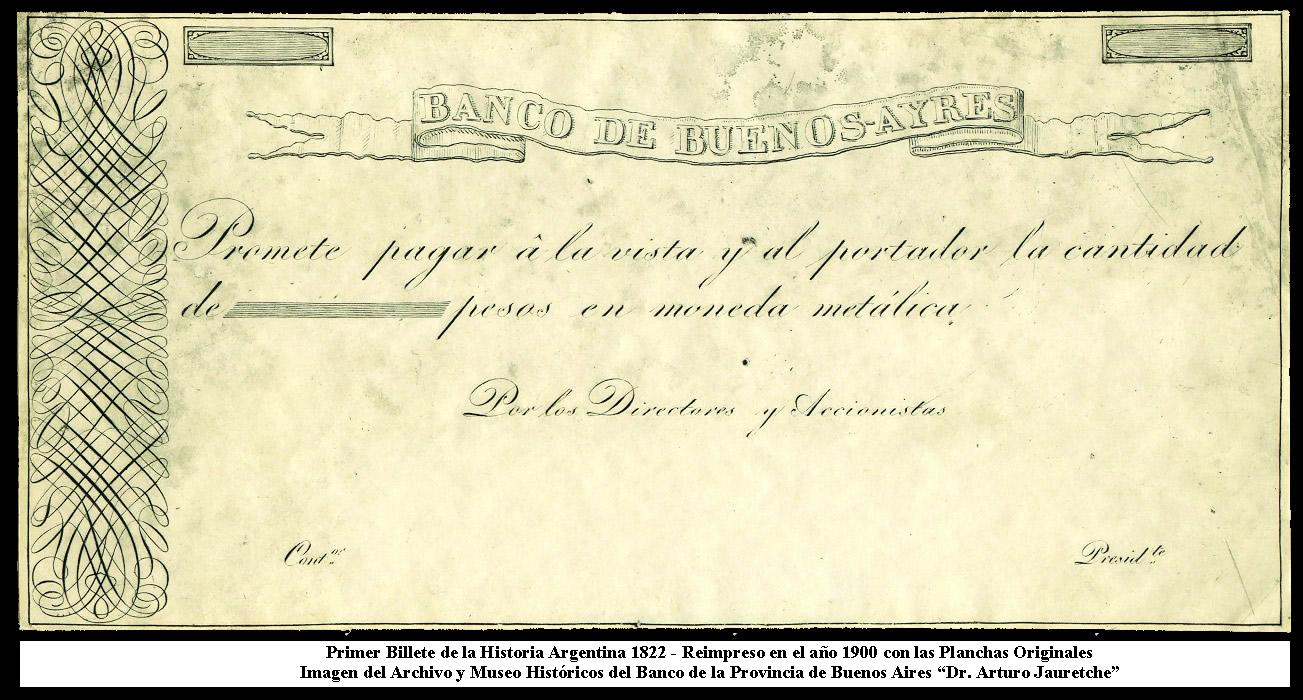
\includegraphics[scale=0.3]{uni1_mon02}
  \caption[bpe]{Primer billete argentino (1822)}
  \label{fig:uni1_01}
\end{figure} 
  \end{frame}

  
\begin{frame}\frametitle{Anarquía monetaria: pre-1880 (cont.)}
     \begin{itemize}
     \item Desde la creación de los primeros billetes, las tensiones
       monetarias y cambiarias empezaron a manifestarse [Banco de
       Descuentos de Buenos Aires situación crítica]
      \item Una de las primeras evidencias de préstamos de un banco de
        emisión al gobierno se encuentra en los inicios del Banco
        Nacional [ex Banco de Descuentos]
        \item Puede observarse un fuerte aumento de la emisión
          coriginada en prestamos al Estado
         \end{itemize}
        \end{frame}


  \begin{frame}\frametitle{Anarquía monetaria: pre-1880 (cont.)}
\begin{figure}[htbp]\vspace{0cm}
  \centering
  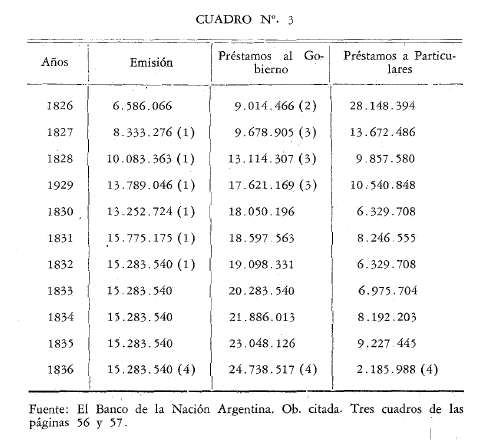
\includegraphics[scale=0.5]{uni1_mon03}
  \caption[bpe]{Emisión monetaria y financiamiento estatal. Fuente:
    Carranza Pérez (1943)}
  \label{fig:uni1_01}
\end{figure} 
  \end{frame}



  \begin{frame}\frametitle{Anarquía monetaria: pre-1880 (cont.)}
\begin{figure}[htbp]\vspace{0cm}
  \centering
  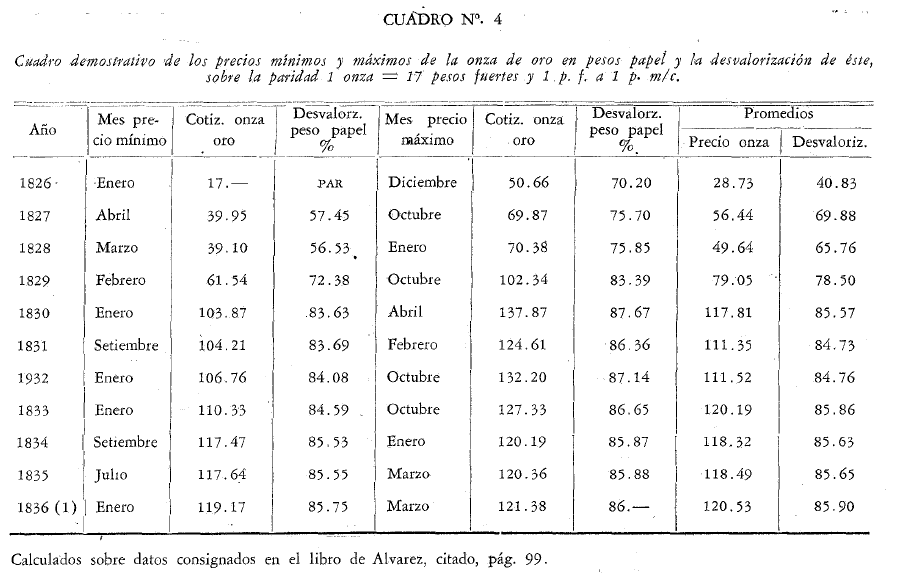
\includegraphics[scale=0.4]{uni1_mon04}
  \caption[bpe]{Depreciación de la moneda local. Fuente: Carranza
    Perez (1943)}
  \label{fig:uni1_01}
\end{figure} 
  \end{frame}

  
\begin{frame}\frametitle{Anarquía monetaria: pre-1880 (cont.)}
     \begin{itemize}
     \item Esa tónica seguiría por los proximos 20-30 años con las
       sucesivas mutaciones del Banco de Descuentos (Banco Nacional
       luego Casa de Moneda)
       \item El dinero metálico es cada vez más escaso --las
         fluctuaciones del billete frente al metálico eran cada vez
         mayores.
         \item La emision monetaria seguía el ritmo de las
           necesidades del Estado
         \end{itemize}
        \end{frame}



        
  \begin{frame}\frametitle{Anarquía monetaria: pre-1880 (cont.)}
\begin{figure}[htbp]\vspace{0cm}
  \centering
  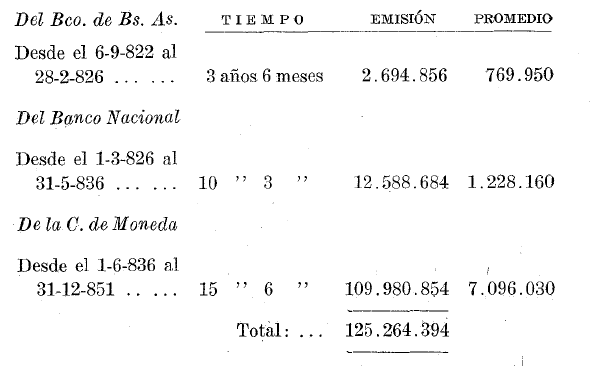
\includegraphics[scale=0.5]{uni1_mon05}
  \caption[bpe]{Aumento de la emisión: 1822-1851 de la moneda local. Fuente: Carranza
    Perez (1943)}
  \label{fig:uni1_01}
\end{figure} 
  \end{frame}


        
  \begin{frame}\frametitle{Anarquía monetaria: pre-1880 (cont.)}
\begin{figure}[htbp]\vspace{0cm}
  \centering
  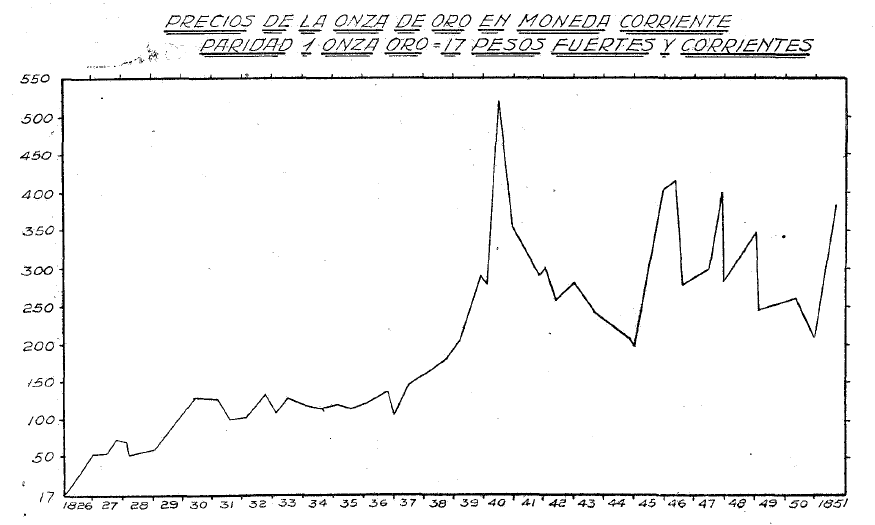
\includegraphics[scale=0.4]{uni1_mon06}
  \caption[bpe]{Depreciación del papel moneda. Fuente: Carranza
    Perez (1943)}
  \label{fig:uni1_01}
\end{figure} 
  \end{frame}

        
  
  

\begin{frame}\frametitle{Anarquía monetaria: pre-1880 (cont.)}
     \begin{itemize}
     \item Cuando Buenos Aires se anexa a la Confederación, el sistema
       monetario era caótico
       \begin{itemize} \itemsep 10pt \bigskip
       \item En Buenos Aires circulaba dinero-papel (emitido por Banco
         de la Provincia de Buenos Aires (BPBA))
         \item En el resto circulaban múltiples
       \textbf{monedas métalicas}: onza hispanoamericana, Cóndor chileno, pesos
       (y centavos) de plata chilenos, bolivianos y peruanos;
       ``melgarejos''; también circulaban billetes provinciales inconvertibles 
     \end{itemize}
   \item No existía unidad monetaria nacional
       \item Se aceptaban
       otras monedas metálicas extranjeras (napoleones, libras,
       aguilas de EEUU y milreis Brasil)
         \end{itemize}
        \end{frame}
        
         

\begin{frame}\frametitle{Anarquía monetaria: pre-1880 (cont.)}
\begin{figure}[htbp]\vspace{0cm}
  \centering
  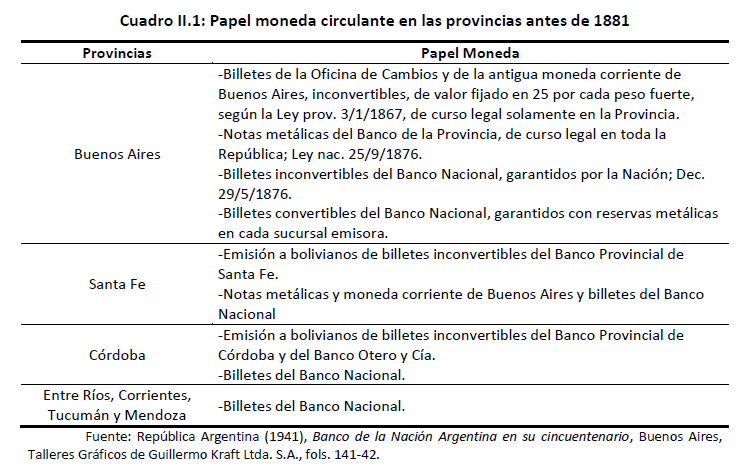
\includegraphics[scale=0.5]{uni1_mon01}
  \caption[bpe]{Tipología de papel moneda circulante pre-1880}
  \label{fig:uni1_01}
\end{figure} 
  \end{frame}


      
\begin{frame}\frametitle{Anarquía monetaria: pre-1880 (cont.)}
\begin{figure}[htbp]\vspace{0cm}
  \centering
  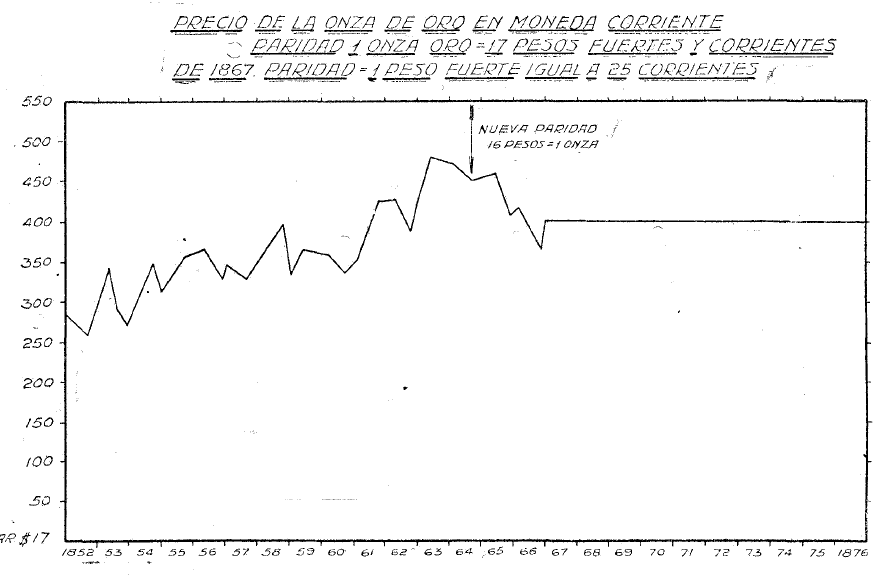
\includegraphics[scale=0.4]{uni1_mon07}
  \caption[bpe]{Depreciación del papel moneda. Fuente: Carranza
    Perez (1943)}
  \label{fig:uni1_01}
\end{figure} 
  \end{frame}

          

\begin{frame}\frametitle{Anarquía monetaria: pre-1880 (cont.)}
     \begin{itemize}
     \item Desde 1860 el BPBA siguió teniendo un control
       principal sobre la política monetaria nacional
       \item Durante este período, el BPBA emitía dinero-papel según
         las necesidades de la epoca --gasto militar en guerras.
         \item Entre 1864 y 1867, pasaron dos cosas: 1) 
           crédito se contrajo; 2) la economía crecía $\longrightarrow$ aprecia peso por
           entrada de K y aumento de tasa de interés real
         \item Convertibilidad y TCFi 1867-1876) $\longrightarrow$ 1 peso fuerte (moneda de
           plata igual a 25 pesos papel)
         \end{itemize}
        \end{frame}
  

\begin{frame}\frametitle{Anarquía monetaria: pre-1880 (cont.)}
\begin{figure}[htbp]\vspace{-0.1cm}
  \centering
  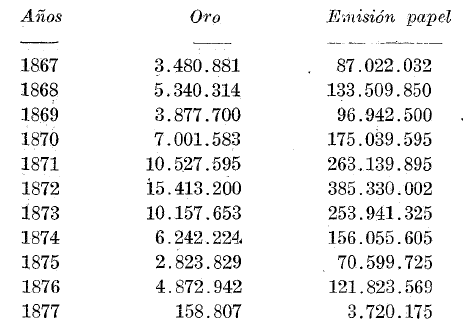
\includegraphics[scale=0.5]{uni1_mon08}
  \caption[bpe]{Dinero metálico y dinero papel,
    1868-77. Fuente: Della Paolera (1994)}
  \label{fig:uni1_01}
\end{figure} 
  \end{frame}


        

\begin{frame}\frametitle{Anarquía monetaria: pre-1880 (cont.)}
\begin{figure}[htbp]\vspace{-0.1cm}
  \centering
  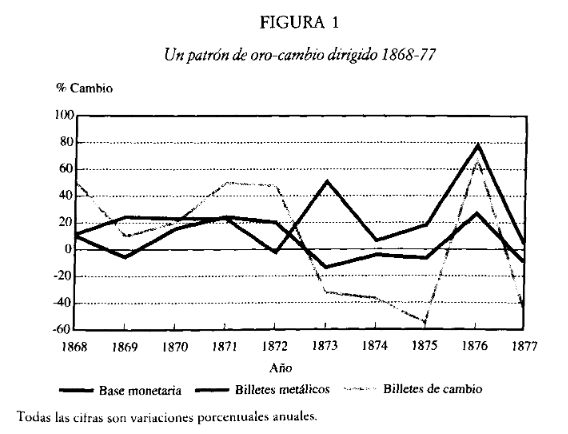
\includegraphics[scale=0.5]{uni2_patron01}
  \caption[bpe]{Base monetaria y circulacion de monedas,
    1868-77. Fuente: Della Paolera (1994)}
  \label{fig:uni1_01}
\end{figure} 
  \end{frame}



\begin{frame}\frametitle{Anarquía monetaria: pre-1880 (cont.)}
     \begin{itemize}
     \item Cuando a partir de 1872-73 se acentúan los saldos
       comerciales y no alcanzan los flujos de K, empieza el drenaje
       de oro
       \item El cociente de reservas a depósitos pasó de 20\% a 3\%
         $\lonrightarrow$ emisión de nuevo dinero metálico impidió el
         colapso de los bancos
         \item En los 55 años entre 1822 y 1877, en que aparece
           primero el billete de banco (luego billete de estado con la
           Casa de Moneda), sólo fue convertible en 13. 
         \end{itemize}
        \end{frame}

  
  
\begin{frame}\frametitle{Unificación monetaria: 1881-1891}
     \begin{itemize}
     \item Ley 1130 (1881) unifica moneda
       nacional. La \textbf{unidad
         monetaria} serían \textbf{peso oro (1.6129 gr y 0.9 pureza)} y \textbf{peso
         plata (25 gr y 0.9 pureza)} sean de curso legal.
       \item Casa de Moneda de la Nación podía acuñar monedas de oro,
         plata y cobre $\longrightarrow$ Argentino de Oro (5 pesos
         moneda nacional) y Patacón de Plata (1 peso moneda nacional)
       \item El papel moneda (emisión) se
         dejó en manos de 5 bancos: Banco Nacional, BPBA, el Banco Provincial de Santa
         Fe, el Banco Provincial de Córdoba y el Banco Otero y Cía. No había restricciones a la emisión fuera de la convertibilidad
         \end{itemize}
        \end{frame}


\begin{frame}\frametitle{Unificación monetaria: 1881-1891 (cont.)}
     \begin{itemize}
     \item A pesar de que la convertibilidad estaba prevista en 1881,
       sólo arrancó hacia fines de 1883.  
     \item  Tenencias metálicas tenían un doble propósito:
       \begin{itemize}\itemsep 10pt \medskip
       \item activo para garantizar convertibilidad de papel moneda
       \item activo para pagar/cancelar deudas pagaderas en metálico
       \end{itemize}
       \item En julio 1883 Argentina tenía un \textbf{patrón mixto
           metálico-fiduciario} $\longrightarrow$ pronto no se podría sostener
         \end{itemize}
        \end{frame}

        

\begin{frame}\frametitle{Unificación monetaria: 1881-1891 (cont.)}
\vspace{-0.5cm}
    \begin{columns}
    \begin{column}{0.4\linewidth}
      \begin{itemize}
        \item En 1883, billetes convertibles a (pagaderos en) moneda nacional
          oro
          \item Emisión no regulada estrictamente
      \end{itemize}
    \end{column}
    \begin{column}{0.6\linewidth}\vspace{-0.25cm}
      \begin{figure}
        \centering
        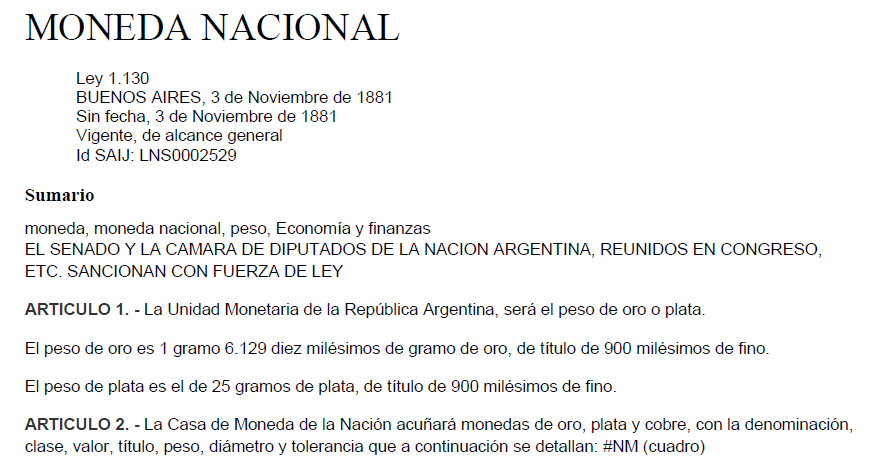
\includegraphics[scale=0.4]{uni2_mon02}
        %\caption{Crecimiento argentino comparado: 1880-1914}
      \end{figure}
    \end{column}
  \end{columns}
  \end{frame}


\begin{frame}\frametitle{Unificación monetaria: 1881-1891 (cont.)}
  \begin{block}{La \textit{Currency School}}
El pensamiento de esta corriente se basa en que la emisión de billetes
debe de estar siempre respaldada por oro. Debe ser ilegal para los
bancos reemplazar billetes por una exportación de oro, sino más bien
deben de reducir sus billetes en la proporción de la exportación de
oro. El pensamiento de esta corriente llevó a la sanción de la
\textit{Peel's Act} en 1844 que restringió la capacidad de emisión de
bancos privados y creó un cuasi-monopolio de emisión del Bank of
England. Efectivamente implica un encaje legal en metálico del 100\%
\end{block}
   \end{frame}



\begin{frame}\frametitle{Unificación monetaria: 1881-1891 (cont.)}
     \begin{itemize}
     \item ¿Cómo funcionaba el negocio bancario?
       \item El \textbf{activo} de un banco estaba compuesto por
         reservas y créditos; en el \textbf{pasivo} estaban los
         billetes en circulación y depósitos. El \textbf{capital
           propio} cerraba el balance
         \item Para emitir 100 pesos papel convertibles a la par en
           pesos oro, debía mantener reservas de metálico en
           proporción (auto) establecida.
           \item Rentabilidad $\longrightarrow$ $r_{B}=i(B-R)$ donde
             $B$ billetes emitidos y $R$ (valor en pesos papel de) reservas metálicas
         \end{itemize}
        \end{frame}


\begin{frame}\frametitle{Unificación monetaria: 1881-1891 (cont.)}
     \begin{itemize}
     \item No es sorprendente que la convertibilidad de pesos papel a
       pesos oro (iniciada en julio de 1883) durara sólo hasta
       diciembre de 1884 $\longrightarrow$ Banco Nacional sin reservas
       \item Decretos de 1885 $\longrightarrow$ autoriza a
         suspender convertibilidad por 2 (dos) años y otorga al papel
         moneda carácter de curso legal.
         \item De un patrón mixto metálico-fiduciario a paridad fija se pasó a un
           patrón fiduciario a paridad flexible
         \end{itemize}
        \end{frame}
        


\begin{frame}\frametitle{Unificación monetaria: 1881-1891 (cont.)}
     \begin{itemize}
     \item Los decretos de 1885 establecieron ciertas restricciones
       por parte de los bancos de emisión:
       \begin{itemize}\itemsep 10pt \medskip
       \item prohibición de disiminuir las reservas metálicas;
         \item obligación de mantener el 50\% de utilidaded liquidas
           anuales en forma de reserva metálica
           \item prohibición de aumentar stock de billetes 
           \end{itemize}
           \item En los meses subsiguientes, varias de estas
             restricciones serían flexibilizadas de hecho y/o derecho
         \end{itemize}
        \end{frame}

        

\begin{frame}\frametitle{Unificación monetaria: 1881-1891 (cont.)}
     \begin{itemize}
     \item Se permitió movilizar los encajes legales en
       metálico $\longrightarrow$ para descuentos en oro, etc; luego
       debían reponerlo
       \item Esto permitió ampliar el negocio bancario! Rentabilidad
         ahora dada por $r_{B}=i(B+R)$
         \item Se prorroga nuevamente la suspensión de la
           convertibilidad hasta 1889; se autoriza nuevas emisiones a bancos de Buenos Aires, Cordoba y Santa Fe (yendo en contra de los decretos de 1885) $\longrightarrow$ en 1886 todas
           las restricciones fijadas en 1885 habían sido levantadas
           y/o flexibilizadas!
         \end{itemize}
        \end{frame}
        
        
        

\begin{frame}\frametitle{Unificación monetaria: 1881-1891 (cont.)}
\begin{figure}[htbp]\vspace{-0.1cm}
  \centering
  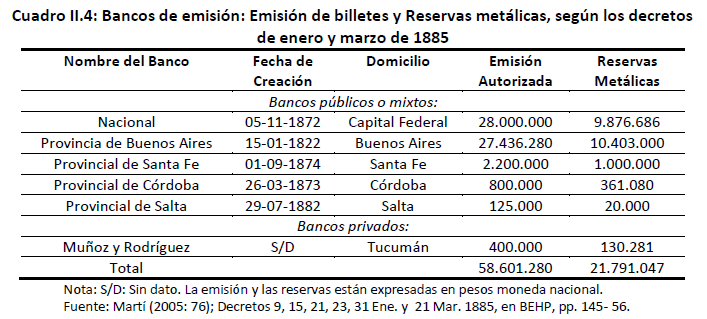
\includegraphics[scale=0.6]{uni2_mon03}
  \caption[bpe]{Emisión de papel y reservas 1885}
  \label{fig:uni1_03}
\end{figure} 
  \end{frame}
        

\begin{frame}\frametitle{Unificación monetaria: 1881-1891 (cont.)}
\begin{figure}[htbp]\vspace{-0.1cm}
  \centering
  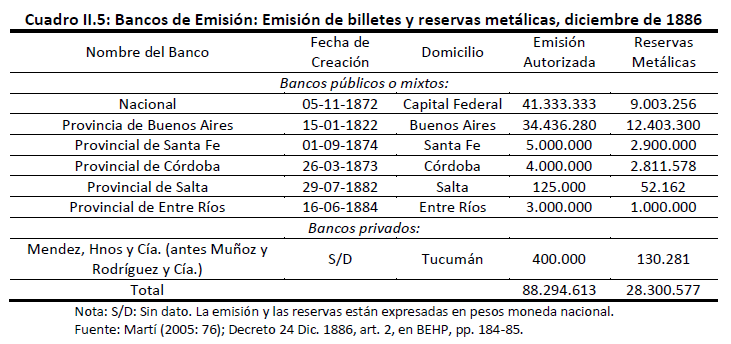
\includegraphics[scale=0.6]{uni2_mon04}
  \caption[bpe]{Emisión de papel y reservas 1886}
  \label{fig:uni1_04}
\end{figure} 
  \end{frame}



\begin{frame}\frametitle{Unificación monetaria: 1881-1891 (cont.)}
     \begin{itemize}
     \item Si comparamos las reservas de metálico en relación a
       emisión entre 1885 y 1886, se observa que había pasado de
       37.2\% a 32\% --no era muy lejano al que autorizaban los
       decretos de 1885
       \item El problema principal es que estas reservas en metálico
         no estaban necesariamente en los bancos sino colocadas como
         activo rentable.
         \item Finalmente, a fines de 1887 se sanciona la \textbf{Ley
             de Bancos Nacionales Garantidos, BNG}.
                \end{itemize}
        \end{frame}




\begin{frame}\frametitle{Unificación monetaria: BNG}
     \begin{itemize}
     \item Disposiciones de la ley de BNG
       \begin{itemize}\itemsep 10pt \bigskip
         \item Todo banco podía emitir papel moneda siempre que
           tuviera 250 mil pesos mon nac. emitiera contra la compra de fondos (títulos) públicos nacionales
         \item Oficina Inspectora (OI) entregaba billetes al banco
           \item Emisión tope $\longrightarrow$ 90\% del capital
             realizado; reserva requerida en oro del 10\% de la emisión, 
             \item Titulos públicos pagaderos en oro a su vencimiento;
               interés del 4.5\% anual $\longrightarrow$ guardados en garantía en OI
               \item 40 millones tope de emisión agregada
               \end{itemize}
               \end{itemize}
        \end{frame}



        \begin{frame}\frametitle{Unificación monetaria: BNG (cont.)}
     \begin{itemize}
     \item Diseño influido por \textit{National Currency Act} de
       EEUU. Implica ir de sistema de múltiples bancos de emisión
       autorizados a bancos libres de emisión
       \item Primer elemento $\longrightarrow$ la emisión implicaba
         crear deuda pública [en EEUU bonos venian de mercados secundarios]
         \item Segundo elemento $\longrightarrow$ bancos no obligados
           a convertir billetes; de hecho no controlaban oferta de
           metálico [en EEUU billetes eran convertibles]
           \item La BM se expandía cuando aumentaba el oro pero no se
             contraía cuando disminuía. 
                \end{itemize}
        \end{frame}


\begin{frame}\frametitle{Unificación monetaria: BNG (cont.)}
\vspace{-0.5cm}
    \begin{columns}
    \begin{column}{0.5\linewidth}
      \begin{figure}
        \centering
        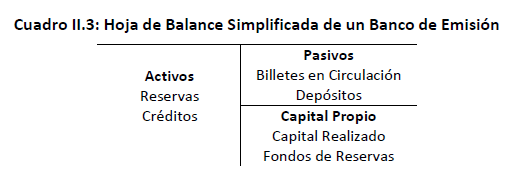
\includegraphics[scale=0.5]{uni1_mon09}
        %\caption{Crecimiento argentino comparado: 1880-1914}
      \end{figure}
    \end{column}
    \begin{column}{0.5\linewidth}\vspace{-0.5cm}
      \begin{figure}
        \centering
        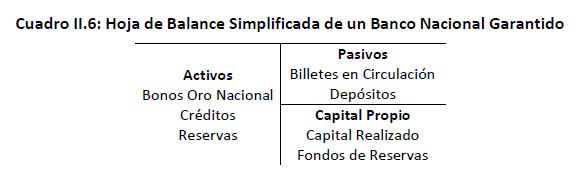
\includegraphics[scale=0.5]{uni1_mon10}
        %\caption{Crecimiento argentino comparado: 1880-1914}
      \end{figure}
    \end{column}
  \end{columns}
  \end{frame}


  
        \begin{frame}\frametitle{Unificación monetaria: BNG (cont.)}
     \begin{itemize}
     \item Para colocar 100 pesos papel el banco debía comprar un
       título público de 100 pesos oro al 85\% de su valor
       $\longrightarrow$ debía disminuir otros activos --reservas y/o
       crédito- para pagar los títulos; alternativamente aumentar el
       capital propio
       \item Rentabilidad ahora dada por $r_{B}=K+i0.9B-iT$ donde $K$
         es el interes anual de los títulos; $B$ emision en pesos
         papel y $T$ valor en pesos papel de los bonos oro
         \item La adhesión de los viejos bancos a la ley de BNG fue absoluta
                \end{itemize}
        \end{frame}




\begin{frame}\frametitle{Unificación monetaria: BNG (cont.)}
\begin{figure}[htbp]\vspace{0cm}
  \centering
  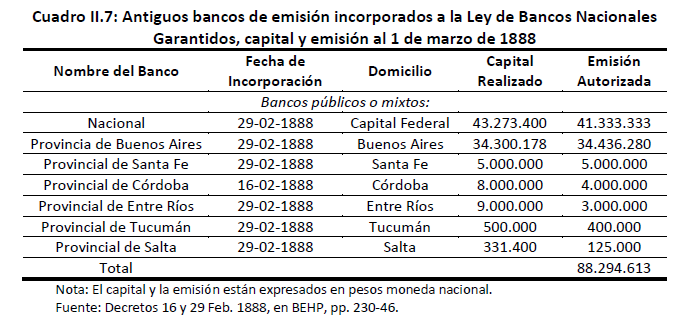
\includegraphics[scale=0.6]{uni1_mon11}
  \caption[bpe]{Antiguos bancos sumados a la ley BNG. Fuente: Gómez (2012)}
  \label{fig:uni1_04}
\end{figure} 
  \end{frame}


 \begin{frame}\frametitle{Unificación monetaria: BNG (cont.)}
     \begin{itemize}
     \item A principios de 1888 había 88.3 millones de billetes autorizados de
       curso legal en todo el país y eran garantizados por títulos
       públicos nacionales en oro por igual valor
       \item A finales de 1888 se conceden nuevas autorizaciones a los
         viejos bancos; del mismo modo, se autoriza a nuevos bancos a
         entrar en el negocio --casi todos fueron a provincias donde
         no había.
                \end{itemize}
        \end{frame}

  


\begin{frame}\frametitle{Unificación monetaria: BNG (cont.)}
\begin{figure}[htbp]\vspace{0cm}
  \centering
  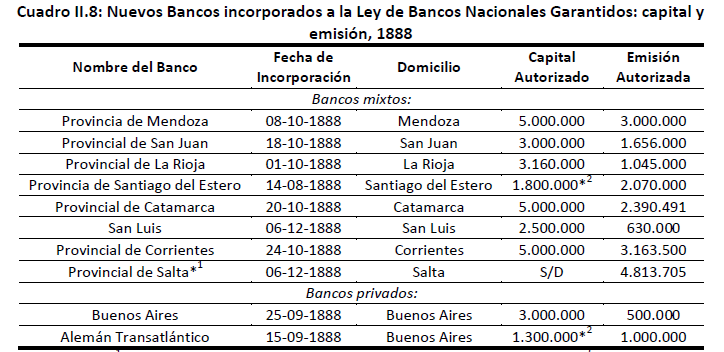
\includegraphics[scale=0.6]{uni1_mon12}
  \caption[bpe]{Nuevos bancos se suman al sistema BNG. Fuente: Gómez (2012)}
  \label{fig:uni1_04}
\end{figure} 
  \end{frame}
        

\begin{frame}\frametitle{Unificación monetaria: BNG (cont.)}
     \begin{itemize}
     \item Muchos de los nuevos bancos (provinciales, mixtos y
       privados) no eran conocidos en absoluto --se aprovecharon de
       liquidez internacional existente. Tomaron deuda afuera para comprar
       los títulos publicos que les permitía emitir
       \item Esencialmente se hacía como una forma de arbitraje
         $\longrightarrow$ el interés de 4.5\% que rendian los titulos
         se usaba para pagar el interés de 6.0\% que se debía a
         acreedores --pero además se obtenían billetes que se
        descontaban (a cambio de un interés) a clientes que le
        otorgaban creditos. El rendimiento era $\r_{B}=K+i0.9B-i^{*}T$ 
                \end{itemize}
        \end{frame}


\begin{frame}\frametitle{Unificación monetaria: BNG (cont.)}
     \begin{itemize}
     \item No debería sorprender que la emisión autorizada aumentó de
       85 a 203 millones pesos mn entre 1888 y 1890 y llegó a un
       maximo de 295 millones de moneda inconvertible
       \item En 1889 más bancos comerciales (creados antes) se incorporan al sistema
         --Gobierno ``incentivó'' a los nuevos bancos a participar al
         amenazar con cobrar un impuesto del 2\% de los depósitos de
         bancos comerciales no adheridos al sistema BNG
         \item De más esta decir que este sistema tuvo impactos sobre
           el valor del peso moneda nacional $\longrightarrow$ en 1891
           caen el Banco Nacional y el BPBA --se funda en 1891 el BNA
                \end{itemize}
        \end{frame}



        \begin{frame}\frametitle{Unificación monetaria: BNG (cont.)}
\begin{figure}[htbp]\vspace{0cm}
  \centering
  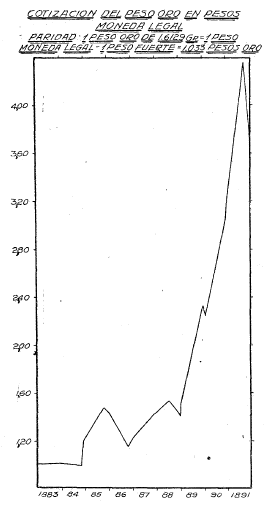
\includegraphics[scale=0.45]{uni1_mon13}
  \caption[bpe]{Depreciación del papel moneda. Fuente: Carranza
    Perez (1943)}\vspace{-0.25cm}
  \label{fig:uni1_04}
\end{figure} 
  \end{frame}
        

  \subsection{Las cuentas fiscales y la política fiscal}

\begin{frame}\frametitle{Las cuentas fiscales}
     \begin{itemize}
     \item Los ingresos del fisco provenían casi exclusivamente del
       comercio exterior --impuestos a las importaciones representaban
       2/3 de los ingresos corrientes
       \item El principal gasto público en esa epoca tenía su origen
         en el Ministerio del Interior (entre un 36 y un 40\%)
         --encargado de toda la obra pública.
         \item Durante toda la década 1880-1890 siempre hubo déficit primario
                \end{itemize}
        \end{frame}
  
  
        \begin{frame}\frametitle{Las cuentas fiscales (cont.)}
\begin{figure}[htbp]\vspace{0cm}
  \centering
  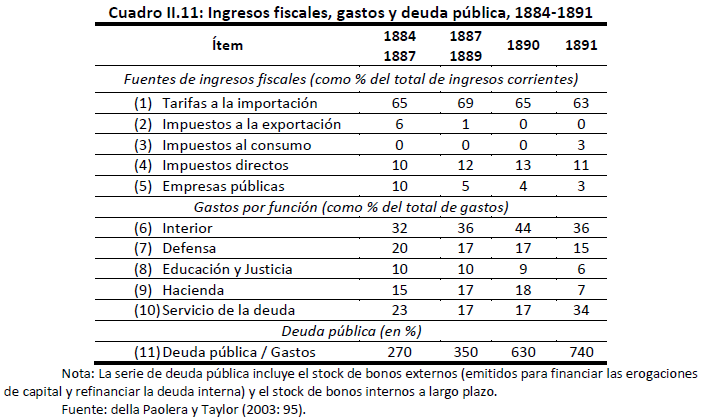
\includegraphics[scale=0.55]{uni1_fis01}
  \caption[bpe]{Ingresos y gastos fiscales - Composición. Fuente:
    Gómez (2012)}\vspace{-0.25cm}
  \label{fig:uni1_04}
\end{figure} 
  \end{frame}
        

 \begin{frame}\frametitle{Las cuentas fiscales (cont.)}
\begin{figure}[htbp]\vspace{0cm}
  \centering
  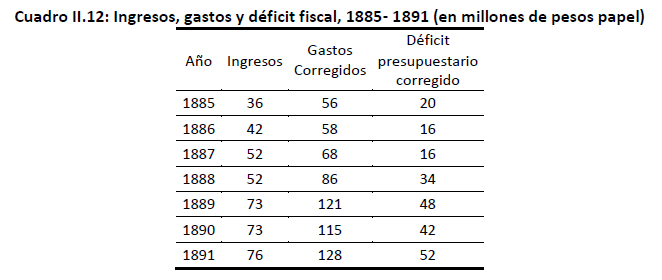
\includegraphics[scale=0.55]{uni1_fis02}
  \caption[bpe]{El déficit fiscal - Evolución. Fuente:
    Gómez (2012)}\vspace{-0.25cm}
  \label{fig:uni1_04}
\end{figure} 
  \end{frame}


  \begin{frame}\frametitle{Financiamiento del déficit}
     \begin{itemize}
     \item Sabemos que el gobierno puede financiar el déficit con: 1)
       venta de bonos publicos (deuda) en mercado de capitales; 2)
       emisión de dinero
       \item Se usa una medida de \textbf{inflación contrafactual} --
         supone que el deficit público se financia 100\% con emision
         \item Si tasa inflacion real similar a contrafactual sugiere
           monetización perfecta del déficit
                \end{itemize}
        \end{frame}


        \begin{frame}\frametitle{Las cuentas fiscales (cont.)}
\begin{figure}[htbp]\vspace{0cm}
  \centering
  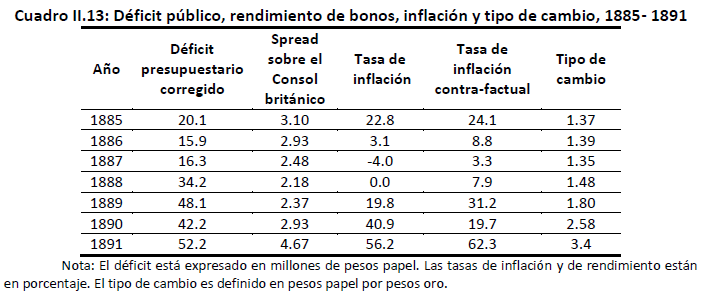
\includegraphics[scale=0.55]{uni1_fis03}
  \caption[bpe]{Deficit, spread e inflación - Evolución. Fuente:
    Gómez (2012)}\vspace{-0.25cm}
  \label{fig:uni1_04}
\end{figure} 
  \end{frame}


 \begin{frame}\frametitle{Las cuentas fiscales (cont.)}
\begin{figure}[htbp]\vspace{0cm}
  \centering
  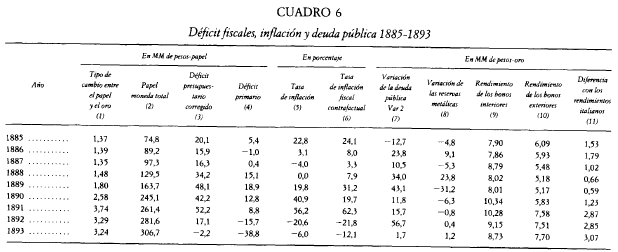
\includegraphics[scale=0.8]{uni1_fis04}
  \caption[bpe]{Deficit, inflación y deuda pública. Fuente:
   Della Paolera (1994))}\vspace{-0.25cm}
  \label{fig:uni1_04}
\end{figure} 
  \end{frame}
  

 \begin{frame}\frametitle{Financiamiento del déficit}
     \begin{itemize}
     \item De las cifras del cuadro se sugiere que en 1885 el deficit
       podía financiarse con emisión; en 1886-88 posiblemente se
       financió deuda al menos parcialmente (ver spread)
       \item Pero a partir de 1888, el deficit fiscal se hizo cada vez
         mas grande, y desde 1889 en adelante, el gobierno tuvo que
         recurrir nuevamente a la emisión monetaria como fuente casi
         exclusiva de financiamiento del déficit $\longrightarrow$
         mayor autonomía monetaria (incovertible) socavó estabilidad
         cambiaria [crisis de 1890-91]
                \end{itemize}
        \end{frame}


  \subsection{La Crisis de 1890-91}


 \begin{frame}\frametitle{La crisis}
     \begin{itemize}
     \item Las primeras señales de debilidad financiera comenzaron en
       1889 en la presidencia de Juárez Celman $\longrightarrow$
       propone pago en pesos papel de deuda con acreedores externos en pesos oro
       \item Primer default parcial --desvaneció crédito externo que
         había sido importante motor de expansión
       \item Paralelamente en Buenos Aires, el público presionaba
         sobre el tipo de cambio demandando pesos oro entregando sus
         pesos papel y se enviaba afuera del país
                \end{itemize}
        \end{frame}



 \begin{frame}\frametitle{La crisis (cont.)}
     \begin{itemize}
     \item Con TCFlex esta salida de oro implicaba depreciacion de la
       moneda local $\longrightarrow$ gobierno nacional intervino para
       evitar depreciación (afectaba precios internos)
     \item La depreciación también afectaba negativamente:
       \begin{itemize}\itemsep 10pt \bigskip
         \item Ingresos fiscales por aranceles a importaciones (baja
           de $M$)
         \item Servicio de pago de la deuda (capital e interés)
         \item Perdida de poder compra de ingresos
         \end{itemize}
       \item Efecto negativo adicional sobre IED y entrada de
         K. Todo esto llevo a adoptar regimen de
           flotación sucia
     \end{itemize}
        \end{frame}



\begin{frame}\frametitle{La crisis (cont.)}
     \begin{itemize}
     \item Se empezó a usar el oro depositado en el Banco Nacional
       --respaldo 'garantía' de todo el sistema bancario- para
       defender el tipo de cambio
       \item Particulares pedían prestamos (pesos papel) para comprar más
         moneda dura (pesos oro) $\longrightarrow$ oro salía de
         circulación
         \item Y esos billetes absorbidos eran luego inyectados
           nuevamente en el circuito $\longrightarrow$ saltó la prima
           del oro en diciembre de 1889 (reservas de oro pasaron de 60
           a 6 millones en 9 meses)
     \end{itemize}
        \end{frame}
        


        \begin{frame}\frametitle{La crisis (cont.)}
     \begin{itemize}
     \item A principios de 1890 \textbf{primera corrida} contra los dos
       principales bancos --Nación y BPBA. El gobierno nacional
       asistió a los bancos y autorizó más emisión no respaldado
       \item Nueva depreciación del peso papel del 20\% impactando en
         precios locales, cuentas públicas y confianza de consumidores
         y empresas
         \item Situacion social agitada (manifestaciones y quejas)
           motivaron cambios en gabinete $\longrightarrow$ se buscó
           salvar a los dos principales bancos. 
     \end{itemize}
  \end{frame}

  
        \begin{frame}\frametitle{La crisis (cont.)}
     \begin{itemize}
     \item Junio 1990 $\longrightarrow$ Banco Nacional anuncia
       suspensión de pago trimestral del servicio de deuda a la
       casa Baring Brothers \& Co $\longrightarrow$ \textbf{segunda corrida}
       bancaria  
\item Crisis política. Renuncia presidente Juárez
  Celman y asume Pellegrini. El nuevo
  ministro de Hacienda (Vicente Lopez) toma 3 importantes medidas:
  1) emisión de 60 mill. en pesos papel de curso legal; 2)
  intervención de bancos de emisión del interior; 3) creación de Caja
  de Conversión.
  \item En tres meses (ago-oct 1890) caído el sistema
    de BNG, el presidente en funciones y se habían
    salvado a los dos principales bancos del país
     \end{itemize}
        \end{frame}

     
        \begin{frame}\frametitle{La crisis (cont.)}
          \begin{block}{El default ante la casa Baring}
            La casa Baring Brothers había suscripto mas de 100 millones
            de pesos oros en títulos de deuda argentinos entre 1882 y
            1890. Entre ellos estaba un empréstito por 25 millones de
            pesos oro de la Buenos Aires Water Supply and Drainage
            Company (1888). La casa Baring Brother se comprometía a
            pagar 21 millones de pesos oro a cambio de bonos por valor
            de 25 millones de pesos oro. Este sería el primer
            \textit{default} de Argentina (segundo si se cuenta el
            primer default de Buenos Aires en 1827)
     \end{block}
        \end{frame}


        
        
        \begin{frame}\frametitle{La crisis (cont.)}
     \begin{itemize}
     \item Se aumentaron impuestos para mejorar las cuentas publicas.
       \item El frente externo --default de la deuda y renegociación-
         seguía aún abierto. De no haber sido por el banco de
         Inglaterra, Baring Brothers hubiera quebrado
         \item Los \textit{fundamentals} macroeconomicos no habian
           mejorado: 1) déficit fiscal aún alto; 2) carga de de la
           deuda muy alta; 2)
           \item Finalmente en 1891 se acuerda el \textbf{empréstito
               de consolidación} $\longrightarrow$ alivio financiero
             en plazos y montos mas requerimientos de ajustes en
             política economica
     \end{itemize}
        \end{frame}

  
        \begin{frame}\frametitle{La crisis (cont.)}
     \begin{itemize}
     \item Ajustes implicaban la imposibilidad por parte del
       gobierno nacional de contraer nuevas deudas y también de
       otorgar nuevos redescuentos a los bancos
       \item El público generó una
         nueva y \textbf{tercera corrida} sobre el Nacional y el
         BPBA que en esta ocasión implicó la caída de ambos (abril 1891) y de casi
         todos los bancos del país
         \item Primer crisis mundial de los mercados emergentes
           $\longrightarrow$ tasa de depreciación del peso papel fue
           de 152.7\% entre 1889 y 1891 y de 270\% entre 1881 y
           1891. La inflación acumulada en el primer período fue de
           163.7\%. 
     \end{itemize}
        \end{frame}



          \subsection{El trilema macroeconómico}

        


        \begin{frame}\frametitle{El trilema macroeconómico}
     \begin{itemize}
     \item El trilema especifica que dados 3 (tres) objetivos de
       política, sólo 2 (dos) pueden ser logrados al mismo
       tiempo y ser simultáneamente consistentes
       \begin{enumerate}\itemsep 10pt \bigskip
                \item tipo de cambio fijo $\longrightarrow$ con motivo
                  de estabilizar precios relativos
                  \item libre movilidad de capitales $\longrightarrow$
                    eficiencia y flexbilidad
                    \item política monetaria activa                      $\longrightarrow$ con motivo de estabilizar el
                      producto
                    \end{enumerate}
                    \item Usar PM activa (3) para desacoplar tasa local de
                      tasa internacional, entonces el arbitraje en
                      mercados de K (2) y la paridad del interés
                      simple (1) haran imposible que se logren las
                      tres cosas (presión sobre TCFi) 
     \end{itemize}
        \end{frame}

          
 \begin{frame}\frametitle{El trilema macroeconómico (cont.)}
\begin{figure}[htbp]\vspace{0cm}
  \centering
  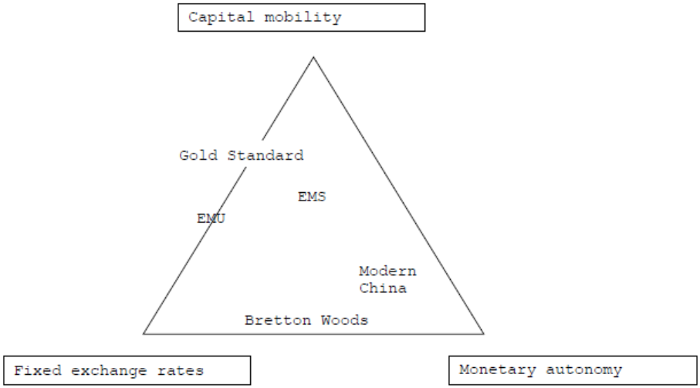
\includegraphics[scale=0.4]{uni1_mon16}
  \caption[bpe]{El trilema macroeconómico clásico)}\vspace{-0.25cm}
  \label{fig:uni1_04}
\end{figure} 
  \end{frame}


  
        \begin{frame}\frametitle{El trilema macroeconómico (cont.)}
     \begin{itemize}
     \item En el período de \textbf{patrón oro clásico}
       --1873 a 1913- los gobiernos de los países habían
       optado por 2 (dos) objetivos: 1) movilidad libre de K; 2) tipo
       de cambio fijo.
       \item Argentina usó (con matices) la misma
         estrategia: convertibilidad de 1881-84,
         intento de retomar conversión en 1885 y ley de BNG en
         1887 $\longrightarrow$ política monetaria endógena
         \item En 1889 se hizo imposible sostener el TCFi --al cortarse el \textbf{crédito externo} la
           única fuente de recursos fiscales era la \textbf{emisión
             monetaria}. 
     \end{itemize}
        \end{frame}
        


           \begin{frame}\frametitle{}
          \begin{block}{El fin de un experimento monetario}
          La fenomenal crisis de 1890-91 significó el (triste) final para uno de
          los primeros experimentos monetarios argentinos --el de la
          unificación monetaria acoplada con convertibilidad monetaria
          y paridad cambiaria. La reversión de los flujos de capitales
          sumada a la creciente emisión de papel moneda incovertible
          (casi exclusivamente para financiar al sector público)
          generó una presión insostenible sobre el tipo de cambio que
          culminó en una crisis típica de mercados emergentes. Con el
          tiempo esta crisis sería una de las mas estudiadas por
          historiadores económicos.
     \end{block}
        \end{frame}

        
        
  
        \end{document}

        